\documentclass[12pt,a4paper]{article}
\synctex=1
\usepackage[utf8]{inputenc}
\usepackage[margin=1cm]{geometry}
\usepackage{graphicx}
%\usepackage{verbatim}
\usepackage{amsmath}
\usepackage{amsfonts}
\usepackage{amssymb}
\usepackage{listings}
\usepackage{enumitem}
\usepackage{textcomp}
\usepackage{courier}
\usepackage{libertine}
\usepackage{pgfornament}
\usepackage{eso-pic}
\usepackage[hangul]{kotex}
\linespread{1.3}

\title{
	\centering
	\pgfornament[width=12cm,color=teal]{84}\\
	\vspace{1cm}
	\fontsize{50}{50} \selectfont {정보통신 수학 및 실습\\Lab assignment}\\
		\pgfornament[width=12cm,color=teal]{88}\\
	\vfill}
\author{
	\LARGE
	\begin{tabular}{rcc}
		\hline
		학번 : & 2016110056 & 2012112130\\ 
		이름 : & 박승원 & 노희승\\
		편성 : & 20조 & \today\\
		\hline
	\end{tabular}\vspace{1cm}
	\\

\includegraphics[width=0.5\textwidth]{logo.jpg}
	}
\date{}

\begin{document}
\maketitle
\pagenumbering{gobble}
\noindent
\lstset{language=matlab, columns=flexible, tabsize=4, frame=shadowbox, showstringspaces=false, breaklines=true, upquote=true, basicstyle=\normalsize}

\renewcommand{\thesubsubsection}{\alph{subsubsection})}
\renewcommand{\thesubsection}{\arabic{subsection}.}
\newpage
\section*{Chapter 11 Lab Assignment}

\subsection{Find the Fourier transform of the following function using the numerical method.\\x(t) = exp(-A*t)u(t); t\textgreater 0}

\begin{gather*}
\int_{-\infty}^{\infty}f(t)e^{-j2\pi ft}dt 
=\int_{-\frac{a}{2}}^{\frac{a}{2}}Ae^{-j2\pi ft}dt
\end{gather*}
\subsubsection{Plot the magnitude of the Fourier Transform of the signal when A=10, a=10.} 
\begin{gather*}
\int_{-5}^{5}10e^{-j2\pi ft}dt = \int_{-5}^{5}10e^{-jwt}dt
=10\left[\frac{e^{-jwt}}{-jw}\right]_{-5}^5
=\frac{10}{-jw}(e^{j5w} - e^{-j5w})
=\frac{10}{-jw}\cdot j2\sin(5w)=\frac{100\sin(5w)}{5w}
\end{gather*}
\subsubsection{Plot the magnitude of the Fourier Transform of the signal when when A=10, a=50 on the top of the figure a.} 
위에서 5를 25로 바꾼다.
\lstinputlisting{1.m}
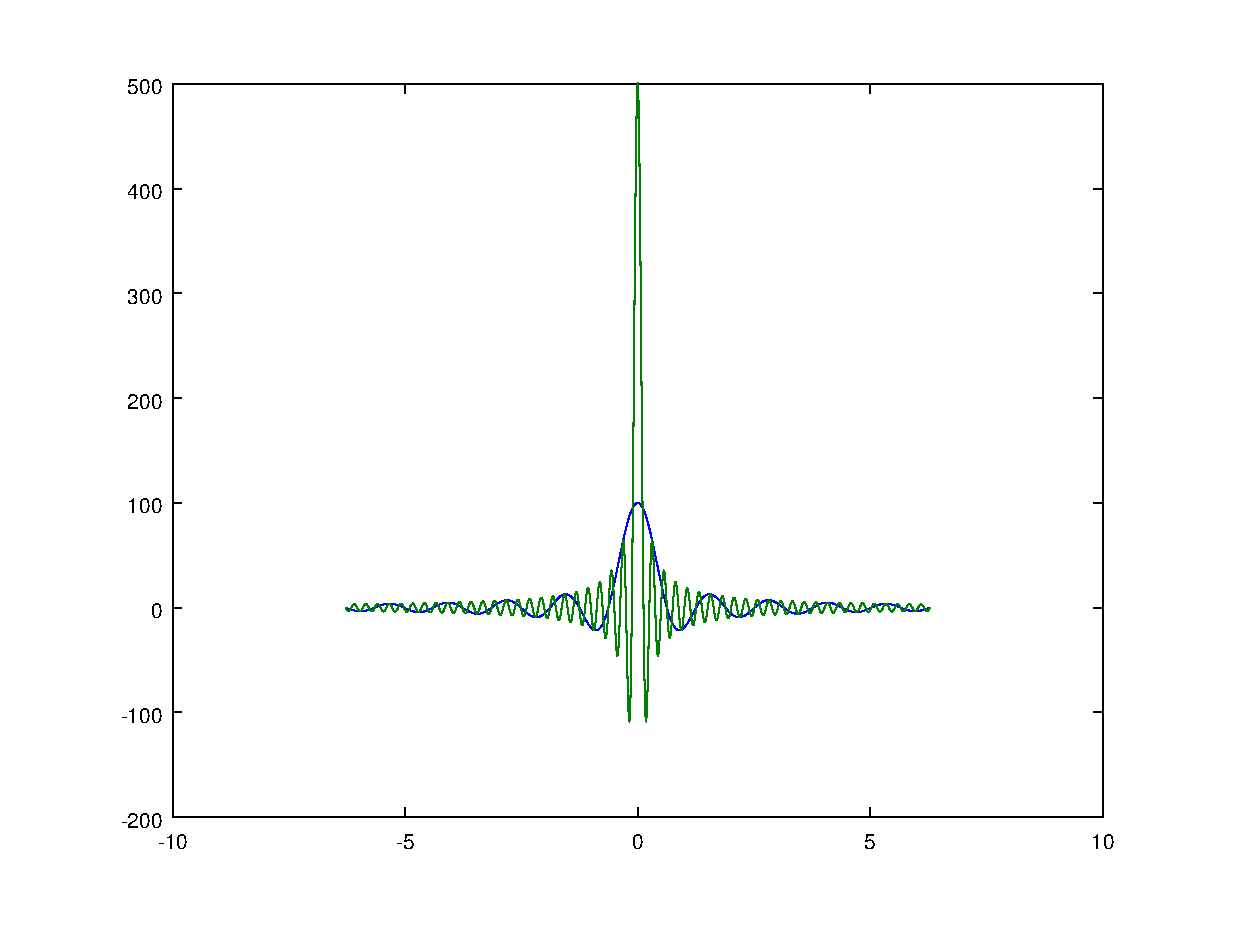
\includegraphics[width=0.8\textwidth]{1.eps}

\subsubsection{Describe what you find through problem a and b.}
time domain에서의 넓은 간격은 frequency domain에서 좁은 저주파 성분이 강한 에너지가 낮은 모양으로 나온다.

\subsection{Solve the following questions about the magnitude of the continuous time Fourier transform of x(t) = exp(-A* abs(t)). Use the numerical method. A is 5.}

\subsubsection{Plot x(t) when -5 \textless t \textless 5.} 
\begin{lstlisting}
t = [-5:0.01:5];
x = exp(-5 * abs(t));
plot(t,x)
\end{lstlisting}
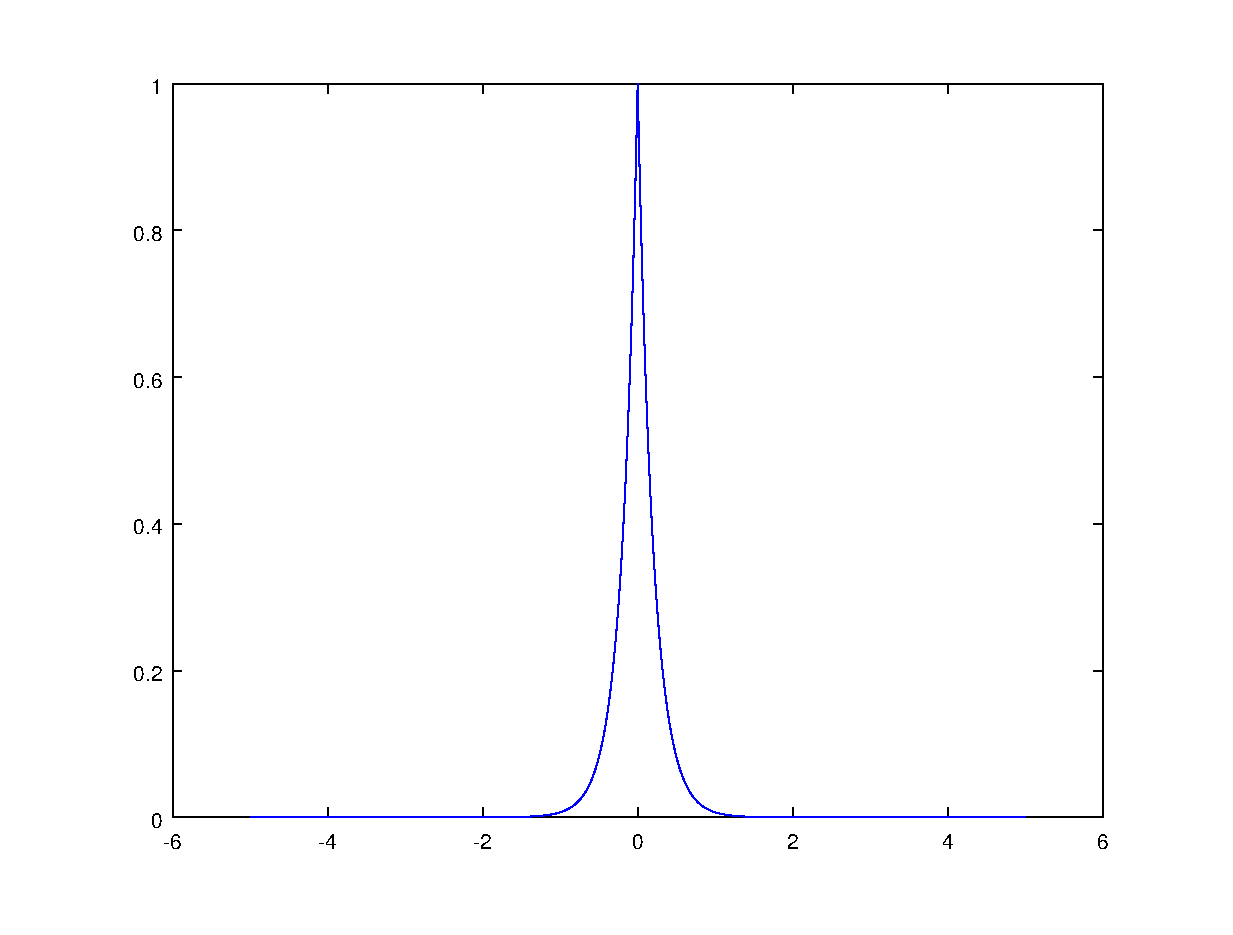
\includegraphics[width=0.8\textwidth]{2.eps}

\subsubsection{Plot the magnitude of the continuous time Fourier transform of x(t) = exp(-A* abs(t)).}
\begin{gather*}
F(f) = \int_{-\infty}^{\infty}e^{-5|t|}e^{-j2\pi ft}dt
\end{gather*}
\lstinputlisting{2.m}
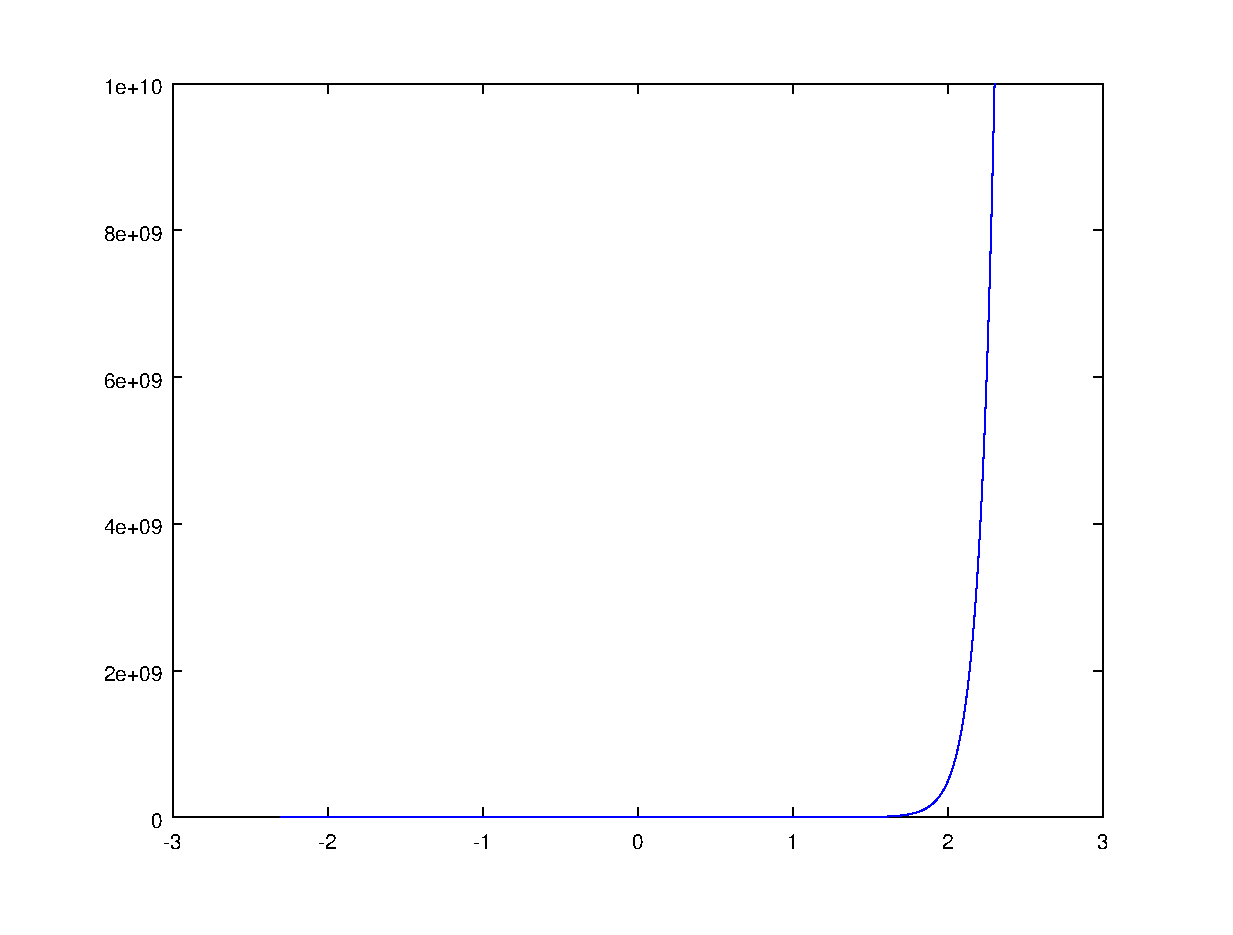
\includegraphics[width=0.8\textwidth]{3.eps}
\subsection{Plot the magnitude of the continuous time Fourier transform of x(t) = 1  when -4 \textless t \textless 4, and x(t)=0 otherwise.} 
\begin{gather*}
\int_{-\infty}^{\infty}e^{-jwt}dt
=\int_{-4}^{4}e^{-jwt}dt
\end{gather*}
\lstinputlisting{3.m}
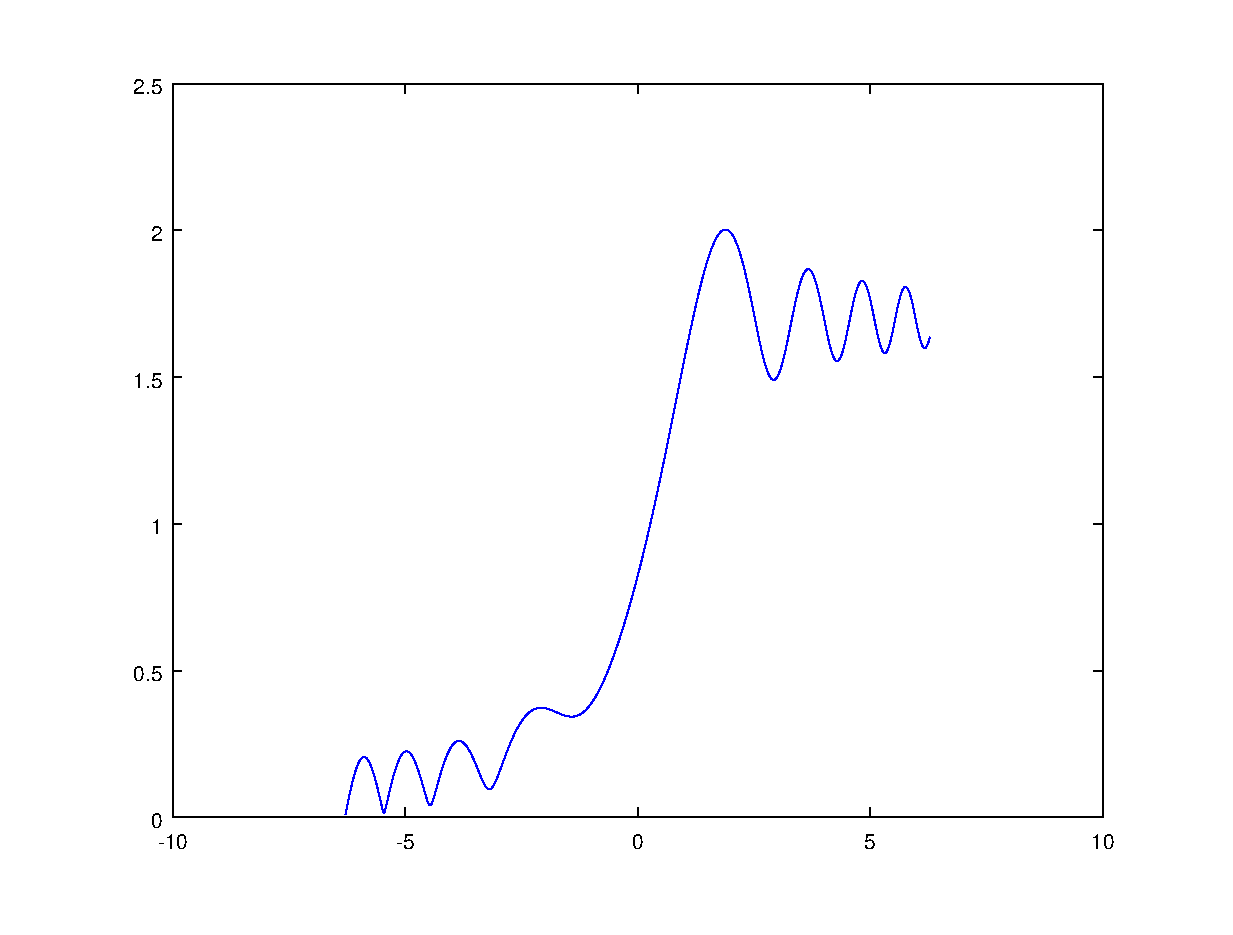
\includegraphics[width=0.8\textwidth]{4.eps}
\end{document}
